% Options for packages loaded elsewhere
\PassOptionsToPackage{unicode}{hyperref}
\PassOptionsToPackage{hyphens}{url}
%
\documentclass[
]{article}
\usepackage{amsmath,amssymb}
\usepackage{lmodern}
\usepackage{ifxetex,ifluatex}
\ifnum 0\ifxetex 1\fi\ifluatex 1\fi=0 % if pdftex
  \usepackage[T1]{fontenc}
  \usepackage[utf8]{inputenc}
  \usepackage{textcomp} % provide euro and other symbols
\else % if luatex or xetex
  \usepackage{unicode-math}
  \defaultfontfeatures{Scale=MatchLowercase}
  \defaultfontfeatures[\rmfamily]{Ligatures=TeX,Scale=1}
\fi
% Use upquote if available, for straight quotes in verbatim environments
\IfFileExists{upquote.sty}{\usepackage{upquote}}{}
\IfFileExists{microtype.sty}{% use microtype if available
  \usepackage[]{microtype}
  \UseMicrotypeSet[protrusion]{basicmath} % disable protrusion for tt fonts
}{}
\makeatletter
\@ifundefined{KOMAClassName}{% if non-KOMA class
  \IfFileExists{parskip.sty}{%
    \usepackage{parskip}
  }{% else
    \setlength{\parindent}{0pt}
    \setlength{\parskip}{6pt plus 2pt minus 1pt}}
}{% if KOMA class
  \KOMAoptions{parskip=half}}
\makeatother
\usepackage{xcolor}
\IfFileExists{xurl.sty}{\usepackage{xurl}}{} % add URL line breaks if available
\IfFileExists{bookmark.sty}{\usepackage{bookmark}}{\usepackage{hyperref}}
\hypersetup{
  pdftitle={BlackGillShrimpDADA2},
  pdfauthor={Jennifer Ouyang},
  hidelinks,
  pdfcreator={LaTeX via pandoc}}
\urlstyle{same} % disable monospaced font for URLs
\usepackage[margin=1in]{geometry}
\usepackage{color}
\usepackage{fancyvrb}
\newcommand{\VerbBar}{|}
\newcommand{\VERB}{\Verb[commandchars=\\\{\}]}
\DefineVerbatimEnvironment{Highlighting}{Verbatim}{commandchars=\\\{\}}
% Add ',fontsize=\small' for more characters per line
\usepackage{framed}
\definecolor{shadecolor}{RGB}{248,248,248}
\newenvironment{Shaded}{\begin{snugshade}}{\end{snugshade}}
\newcommand{\AlertTok}[1]{\textcolor[rgb]{0.94,0.16,0.16}{#1}}
\newcommand{\AnnotationTok}[1]{\textcolor[rgb]{0.56,0.35,0.01}{\textbf{\textit{#1}}}}
\newcommand{\AttributeTok}[1]{\textcolor[rgb]{0.77,0.63,0.00}{#1}}
\newcommand{\BaseNTok}[1]{\textcolor[rgb]{0.00,0.00,0.81}{#1}}
\newcommand{\BuiltInTok}[1]{#1}
\newcommand{\CharTok}[1]{\textcolor[rgb]{0.31,0.60,0.02}{#1}}
\newcommand{\CommentTok}[1]{\textcolor[rgb]{0.56,0.35,0.01}{\textit{#1}}}
\newcommand{\CommentVarTok}[1]{\textcolor[rgb]{0.56,0.35,0.01}{\textbf{\textit{#1}}}}
\newcommand{\ConstantTok}[1]{\textcolor[rgb]{0.00,0.00,0.00}{#1}}
\newcommand{\ControlFlowTok}[1]{\textcolor[rgb]{0.13,0.29,0.53}{\textbf{#1}}}
\newcommand{\DataTypeTok}[1]{\textcolor[rgb]{0.13,0.29,0.53}{#1}}
\newcommand{\DecValTok}[1]{\textcolor[rgb]{0.00,0.00,0.81}{#1}}
\newcommand{\DocumentationTok}[1]{\textcolor[rgb]{0.56,0.35,0.01}{\textbf{\textit{#1}}}}
\newcommand{\ErrorTok}[1]{\textcolor[rgb]{0.64,0.00,0.00}{\textbf{#1}}}
\newcommand{\ExtensionTok}[1]{#1}
\newcommand{\FloatTok}[1]{\textcolor[rgb]{0.00,0.00,0.81}{#1}}
\newcommand{\FunctionTok}[1]{\textcolor[rgb]{0.00,0.00,0.00}{#1}}
\newcommand{\ImportTok}[1]{#1}
\newcommand{\InformationTok}[1]{\textcolor[rgb]{0.56,0.35,0.01}{\textbf{\textit{#1}}}}
\newcommand{\KeywordTok}[1]{\textcolor[rgb]{0.13,0.29,0.53}{\textbf{#1}}}
\newcommand{\NormalTok}[1]{#1}
\newcommand{\OperatorTok}[1]{\textcolor[rgb]{0.81,0.36,0.00}{\textbf{#1}}}
\newcommand{\OtherTok}[1]{\textcolor[rgb]{0.56,0.35,0.01}{#1}}
\newcommand{\PreprocessorTok}[1]{\textcolor[rgb]{0.56,0.35,0.01}{\textit{#1}}}
\newcommand{\RegionMarkerTok}[1]{#1}
\newcommand{\SpecialCharTok}[1]{\textcolor[rgb]{0.00,0.00,0.00}{#1}}
\newcommand{\SpecialStringTok}[1]{\textcolor[rgb]{0.31,0.60,0.02}{#1}}
\newcommand{\StringTok}[1]{\textcolor[rgb]{0.31,0.60,0.02}{#1}}
\newcommand{\VariableTok}[1]{\textcolor[rgb]{0.00,0.00,0.00}{#1}}
\newcommand{\VerbatimStringTok}[1]{\textcolor[rgb]{0.31,0.60,0.02}{#1}}
\newcommand{\WarningTok}[1]{\textcolor[rgb]{0.56,0.35,0.01}{\textbf{\textit{#1}}}}
\usepackage{graphicx}
\makeatletter
\def\maxwidth{\ifdim\Gin@nat@width>\linewidth\linewidth\else\Gin@nat@width\fi}
\def\maxheight{\ifdim\Gin@nat@height>\textheight\textheight\else\Gin@nat@height\fi}
\makeatother
% Scale images if necessary, so that they will not overflow the page
% margins by default, and it is still possible to overwrite the defaults
% using explicit options in \includegraphics[width, height, ...]{}
\setkeys{Gin}{width=\maxwidth,height=\maxheight,keepaspectratio}
% Set default figure placement to htbp
\makeatletter
\def\fps@figure{htbp}
\makeatother
\setlength{\emergencystretch}{3em} % prevent overfull lines
\providecommand{\tightlist}{%
  \setlength{\itemsep}{0pt}\setlength{\parskip}{0pt}}
\setcounter{secnumdepth}{-\maxdimen} % remove section numbering
\ifluatex
  \usepackage{selnolig}  % disable illegal ligatures
\fi

\title{BlackGillShrimpDADA2}
\author{Jennifer Ouyang}
\date{}

\begin{document}
\maketitle

\begin{Shaded}
\begin{Highlighting}[]
\FunctionTok{library}\NormalTok{(dada2); }\FunctionTok{packageVersion}\NormalTok{(}\StringTok{"dada2"}\NormalTok{)}
\end{Highlighting}
\end{Shaded}

\begin{verbatim}
## Loading required package: Rcpp
\end{verbatim}

\begin{verbatim}
## Warning: package 'Rcpp' was built under R version 4.0.5
\end{verbatim}

\begin{verbatim}
## [1] '1.18.0'
\end{verbatim}

\begin{Shaded}
\begin{Highlighting}[]
\NormalTok{path }\OtherTok{\textless{}{-}} \StringTok{"C:/Users/Jennifer Ouyang/RStudio/MarineLab/src"}
\FunctionTok{list.files}\NormalTok{(path)}
\end{Highlighting}
\end{Shaded}

\begin{verbatim}
##  [1] "165_S159_L001_R1_001.fastq"                
##  [2] "165_S159_L001_R2_001.fastq"                
##  [3] "166_S160_L001_R1_001.fastq"                
##  [4] "166_S160_L001_R2_001.fastq"                
##  [5] "167_S161_L001_R1_001.fastq"                
##  [6] "167_S161_L001_R2_001.fastq"                
##  [7] "168_S162_L001_R1_001.fastq"                
##  [8] "168_S162_L001_R2_001.fastq"                
##  [9] "169_S163_L001_R1_001.fastq"                
## [10] "169_S163_L001_R2_001.fastq"                
## [11] "170_S164_L001_R1_001.fastq"                
## [12] "170_S164_L001_R2_001.fastq"                
## [13] "171_S165_L001_R1_001.fastq"                
## [14] "171_S165_L001_R2_001.fastq"                
## [15] "173_S166_L001_R1_001.fastq"                
## [16] "173_S166_L001_R2_001.fastq"                
## [17] "174_S167_L001_R1_001.fastq"                
## [18] "174_S167_L001_R2_001.fastq"                
## [19] "175_S168_L001_R1_001.fastq"                
## [20] "175_S168_L001_R2_001.fastq"                
## [21] "176_S169_L001_R1_001.fastq"                
## [22] "176_S169_L001_R2_001.fastq"                
## [23] "177_S170_L001_R1_001.fastq"                
## [24] "177_S170_L001_R2_001.fastq"                
## [25] "178_S171_L001_R1_001.fastq"                
## [26] "178_S171_L001_R2_001.fastq"                
## [27] "179_S172_L001_R1_001.fastq"                
## [28] "179_S172_L001_R2_001.fastq"                
## [29] "180_S173_L001_R1_001.fastq"                
## [30] "180_S173_L001_R2_001.fastq"                
## [31] "181_S174_L001_R1_001.fastq"                
## [32] "181_S174_L001_R2_001.fastq"                
## [33] "182_S175_L001_R1_001.fastq"                
## [34] "182_S175_L001_R2_001.fastq"                
## [35] "183_S176_L001_R1_001.fastq"                
## [36] "183_S176_L001_R2_001.fastq"                
## [37] "184_S177_L001_R1_001.fastq"                
## [38] "184_S177_L001_R2_001.fastq"                
## [39] "filtered"                                  
## [40] "silva_nr99_v138.1_train_set.fa.gz"         
## [41] "silva_nr99_v138.1_wSpecies_train_set.fa.gz"
\end{verbatim}

\begin{Shaded}
\begin{Highlighting}[]
\CommentTok{\# Forward and reverse fastq filenames have format: SAMPLENAME\_R1\_001.fastq and SAMPLENAME\_R2\_001.fastq}
\NormalTok{fnFs }\OtherTok{\textless{}{-}} \FunctionTok{sort}\NormalTok{(}\FunctionTok{list.files}\NormalTok{(path, }\AttributeTok{pattern=}\StringTok{"\_R1\_001.fastq"}\NormalTok{, }\AttributeTok{full.names =} \ConstantTok{TRUE}\NormalTok{))}
\NormalTok{fnRs }\OtherTok{\textless{}{-}} \FunctionTok{sort}\NormalTok{(}\FunctionTok{list.files}\NormalTok{(path, }\AttributeTok{pattern=}\StringTok{"\_R2\_001.fastq"}\NormalTok{, }\AttributeTok{full.names =} \ConstantTok{TRUE}\NormalTok{))}
\CommentTok{\# Extract sample names, assuming filenames have format: SAMPLENAME\_XXX.fastq}
\NormalTok{sample.names }\OtherTok{\textless{}{-}} \FunctionTok{sapply}\NormalTok{(}\FunctionTok{strsplit}\NormalTok{(}\FunctionTok{basename}\NormalTok{(fnFs), }\StringTok{"\_"}\NormalTok{), }\StringTok{\textasciigrave{}}\AttributeTok{[}\StringTok{\textasciigrave{}}\NormalTok{, }\DecValTok{1}\NormalTok{)}
\end{Highlighting}
\end{Shaded}

\#\#Inspect read quality profiles

\begin{Shaded}
\begin{Highlighting}[]
\FunctionTok{plotQualityProfile}\NormalTok{(fnFs[}\DecValTok{1}\SpecialCharTok{:}\DecValTok{2}\NormalTok{])}
\end{Highlighting}
\end{Shaded}

\begin{verbatim}
## Warning: `guides(<scale> = FALSE)` is deprecated. Please use `guides(<scale> =
## "none")` instead.
\end{verbatim}

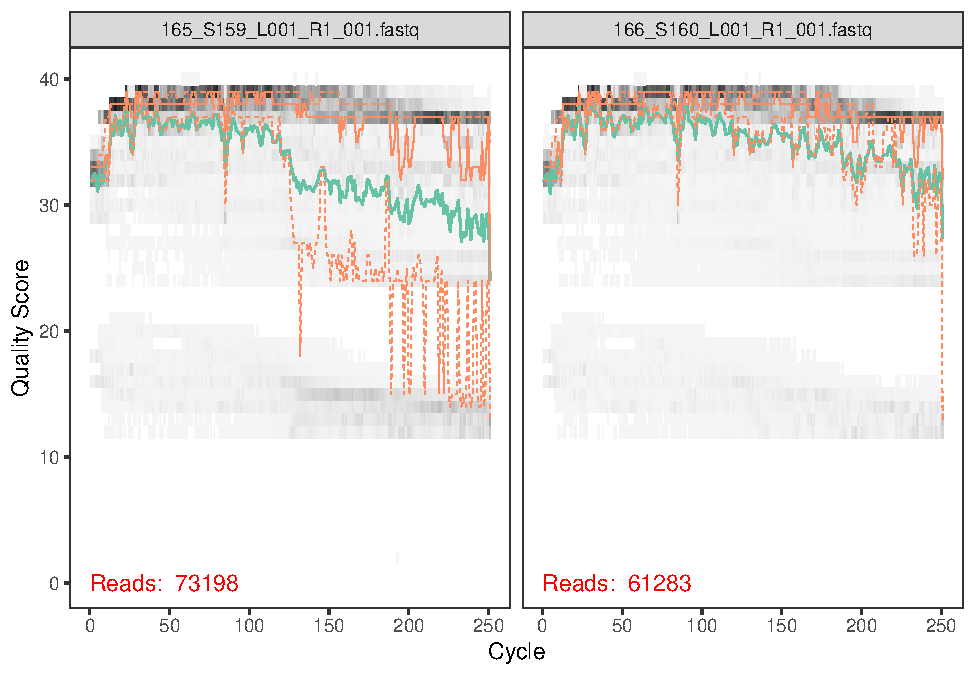
\includegraphics{BlackGillShrimpDADA2_files/figure-latex/unnamed-chunk-2-1.pdf}

\begin{Shaded}
\begin{Highlighting}[]
\FunctionTok{plotQualityProfile}\NormalTok{(fnRs[}\DecValTok{1}\SpecialCharTok{:}\DecValTok{2}\NormalTok{])}
\end{Highlighting}
\end{Shaded}

\begin{verbatim}
## Warning: `guides(<scale> = FALSE)` is deprecated. Please use `guides(<scale> =
## "none")` instead.
\end{verbatim}

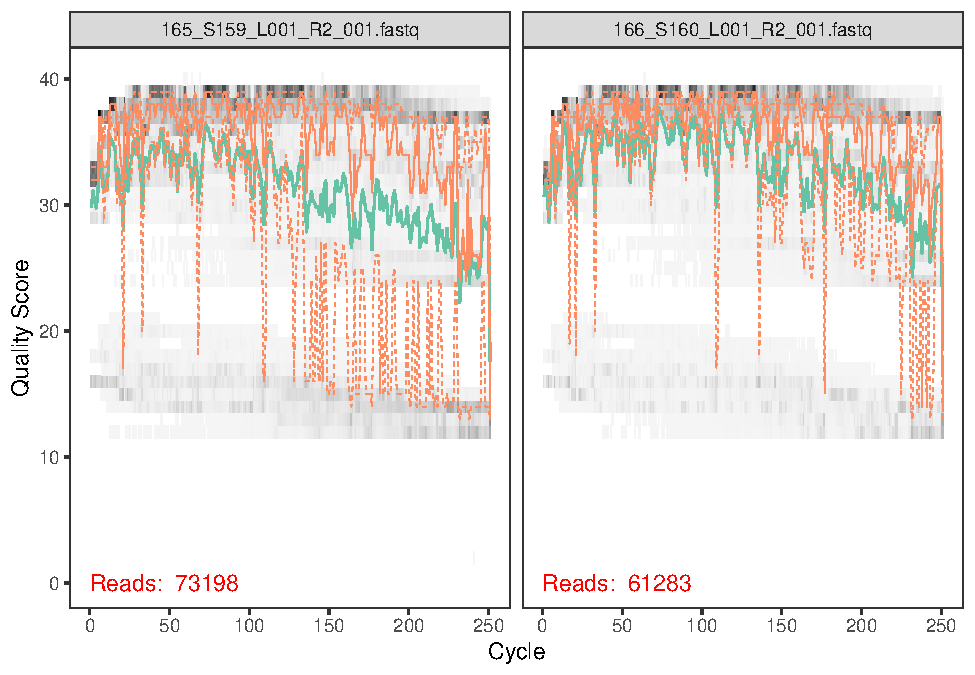
\includegraphics{BlackGillShrimpDADA2_files/figure-latex/unnamed-chunk-3-1.pdf}

\#\#Filter and trim

\begin{Shaded}
\begin{Highlighting}[]
\CommentTok{\# Place filtered files in filtered/ subdirectory}
\NormalTok{filtFs }\OtherTok{\textless{}{-}} \FunctionTok{file.path}\NormalTok{(path, }\StringTok{"filtered"}\NormalTok{, }\FunctionTok{paste0}\NormalTok{(sample.names, }\StringTok{"\_F\_filt.fastq.gz"}\NormalTok{))}
\NormalTok{filtRs }\OtherTok{\textless{}{-}} \FunctionTok{file.path}\NormalTok{(path, }\StringTok{"filtered"}\NormalTok{, }\FunctionTok{paste0}\NormalTok{(sample.names, }\StringTok{"\_R\_filt.fastq.gz"}\NormalTok{))}
\FunctionTok{names}\NormalTok{(filtFs) }\OtherTok{\textless{}{-}}\NormalTok{ sample.names}
\FunctionTok{names}\NormalTok{(filtRs) }\OtherTok{\textless{}{-}}\NormalTok{ sample.names}
\end{Highlighting}
\end{Shaded}

\begin{Shaded}
\begin{Highlighting}[]
\NormalTok{out }\OtherTok{\textless{}{-}} \FunctionTok{filterAndTrim}\NormalTok{(fnFs, filtFs, fnRs, filtRs, }\AttributeTok{truncLen=}\FunctionTok{c}\NormalTok{(}\DecValTok{240}\NormalTok{,}\DecValTok{230}\NormalTok{),}
              \AttributeTok{maxN=}\DecValTok{0}\NormalTok{, }\AttributeTok{maxEE=}\FunctionTok{c}\NormalTok{(}\DecValTok{2}\NormalTok{,}\DecValTok{2}\NormalTok{), }\AttributeTok{truncQ=}\DecValTok{2}\NormalTok{, }\AttributeTok{rm.phix=}\ConstantTok{TRUE}\NormalTok{,}
              \AttributeTok{compress=}\ConstantTok{TRUE}\NormalTok{, }\AttributeTok{multithread=}\ConstantTok{FALSE}\NormalTok{) }\CommentTok{\# On Windows set multithread=FALSE}
\FunctionTok{head}\NormalTok{(out)}
\end{Highlighting}
\end{Shaded}

\begin{verbatim}
##                            reads.in reads.out
## 165_S159_L001_R1_001.fastq    73198     48982
## 166_S160_L001_R1_001.fastq    61283     50361
## 167_S161_L001_R1_001.fastq    76932     64350
## 168_S162_L001_R1_001.fastq    48740     41065
## 169_S163_L001_R1_001.fastq   127769    109440
## 170_S164_L001_R1_001.fastq    75110     62672
\end{verbatim}

\#\#Learn the Error Rates

\begin{Shaded}
\begin{Highlighting}[]
\NormalTok{errF }\OtherTok{\textless{}{-}} \FunctionTok{learnErrors}\NormalTok{(filtFs, }\AttributeTok{multithread=}\ConstantTok{TRUE}\NormalTok{)}
\end{Highlighting}
\end{Shaded}

\begin{verbatim}
## 102606480 total bases in 427527 reads from 7 samples will be used for learning the error rates.
\end{verbatim}

\begin{Shaded}
\begin{Highlighting}[]
\NormalTok{errR }\OtherTok{\textless{}{-}} \FunctionTok{learnErrors}\NormalTok{(filtRs, }\AttributeTok{multithread=}\ConstantTok{TRUE}\NormalTok{)}
\end{Highlighting}
\end{Shaded}

\begin{verbatim}
## 103501380 total bases in 450006 reads from 8 samples will be used for learning the error rates.
\end{verbatim}

\begin{Shaded}
\begin{Highlighting}[]
\FunctionTok{plotErrors}\NormalTok{(errF, }\AttributeTok{nominalQ=}\ConstantTok{TRUE}\NormalTok{)}
\end{Highlighting}
\end{Shaded}

\begin{verbatim}
## Warning: Transformation introduced infinite values in continuous y-axis

## Warning: Transformation introduced infinite values in continuous y-axis
\end{verbatim}

\includegraphics{BlackGillShrimpDADA2_files/figure-latex/unnamed-chunk-8-1.pdf}

\#\#Sample Inference

\begin{Shaded}
\begin{Highlighting}[]
\NormalTok{dadaFs }\OtherTok{\textless{}{-}} \FunctionTok{dada}\NormalTok{(filtFs, }\AttributeTok{err=}\NormalTok{errF, }\AttributeTok{multithread=}\ConstantTok{TRUE}\NormalTok{)}
\end{Highlighting}
\end{Shaded}

\begin{verbatim}
## Sample 1 - 48982 reads in 14907 unique sequences.
## Sample 2 - 50361 reads in 14626 unique sequences.
## Sample 3 - 64350 reads in 17582 unique sequences.
## Sample 4 - 41065 reads in 11632 unique sequences.
## Sample 5 - 109440 reads in 29474 unique sequences.
## Sample 6 - 62672 reads in 18713 unique sequences.
## Sample 7 - 50657 reads in 16149 unique sequences.
## Sample 8 - 22479 reads in 7495 unique sequences.
## Sample 9 - 36027 reads in 10305 unique sequences.
## Sample 10 - 66127 reads in 21660 unique sequences.
## Sample 11 - 54708 reads in 15989 unique sequences.
## Sample 12 - 62654 reads in 19449 unique sequences.
## Sample 13 - 65350 reads in 21761 unique sequences.
## Sample 14 - 83940 reads in 24774 unique sequences.
## Sample 15 - 69538 reads in 18799 unique sequences.
## Sample 16 - 72325 reads in 24100 unique sequences.
## Sample 17 - 76173 reads in 20014 unique sequences.
## Sample 18 - 68599 reads in 19547 unique sequences.
## Sample 19 - 41300 reads in 9692 unique sequences.
\end{verbatim}

\begin{Shaded}
\begin{Highlighting}[]
\NormalTok{dadaRs }\OtherTok{\textless{}{-}} \FunctionTok{dada}\NormalTok{(filtRs, }\AttributeTok{err=}\NormalTok{errR, }\AttributeTok{multithread=}\ConstantTok{TRUE}\NormalTok{)}
\end{Highlighting}
\end{Shaded}

\begin{verbatim}
## Sample 1 - 48982 reads in 19986 unique sequences.
## Sample 2 - 50361 reads in 21466 unique sequences.
## Sample 3 - 64350 reads in 25635 unique sequences.
## Sample 4 - 41065 reads in 15918 unique sequences.
## Sample 5 - 109440 reads in 42988 unique sequences.
## Sample 6 - 62672 reads in 25924 unique sequences.
## Sample 7 - 50657 reads in 21154 unique sequences.
## Sample 8 - 22479 reads in 10559 unique sequences.
## Sample 9 - 36027 reads in 16289 unique sequences.
## Sample 10 - 66127 reads in 26857 unique sequences.
## Sample 11 - 54708 reads in 29154 unique sequences.
## Sample 12 - 62654 reads in 29403 unique sequences.
## Sample 13 - 65350 reads in 30950 unique sequences.
## Sample 14 - 83940 reads in 30903 unique sequences.
## Sample 15 - 69538 reads in 31955 unique sequences.
## Sample 16 - 72325 reads in 31168 unique sequences.
## Sample 17 - 76173 reads in 32970 unique sequences.
## Sample 18 - 68599 reads in 27136 unique sequences.
## Sample 19 - 41300 reads in 13662 unique sequences.
\end{verbatim}

\begin{Shaded}
\begin{Highlighting}[]
\NormalTok{dadaFs[[}\DecValTok{1}\NormalTok{]]}
\end{Highlighting}
\end{Shaded}

\begin{verbatim}
## dada-class: object describing DADA2 denoising results
## 250 sequence variants were inferred from 14907 input unique sequences.
## Key parameters: OMEGA_A = 1e-40, OMEGA_C = 1e-40, BAND_SIZE = 16
\end{verbatim}

\#\#Merge paired reads

\begin{Shaded}
\begin{Highlighting}[]
\NormalTok{mergers }\OtherTok{\textless{}{-}} \FunctionTok{mergePairs}\NormalTok{(dadaFs, filtFs, dadaRs, filtRs, }\AttributeTok{verbose=}\ConstantTok{TRUE}\NormalTok{)}
\end{Highlighting}
\end{Shaded}

\begin{verbatim}
## 48459 paired-reads (in 260 unique pairings) successfully merged out of 48684 (in 310 pairings) input.
\end{verbatim}

\begin{verbatim}
## 48377 paired-reads (in 575 unique pairings) successfully merged out of 49495 (in 792 pairings) input.
\end{verbatim}

\begin{verbatim}
## 62276 paired-reads (in 428 unique pairings) successfully merged out of 63403 (in 651 pairings) input.
\end{verbatim}

\begin{verbatim}
## 40365 paired-reads (in 294 unique pairings) successfully merged out of 40770 (in 381 pairings) input.
\end{verbatim}

\begin{verbatim}
## 106028 paired-reads (in 683 unique pairings) successfully merged out of 107788 (in 1063 pairings) input.
\end{verbatim}

\begin{verbatim}
## 61224 paired-reads (in 532 unique pairings) successfully merged out of 61889 (in 673 pairings) input.
\end{verbatim}

\begin{verbatim}
## 48763 paired-reads (in 437 unique pairings) successfully merged out of 49799 (in 642 pairings) input.
\end{verbatim}

\begin{verbatim}
## 21293 paired-reads (in 313 unique pairings) successfully merged out of 21948 (in 429 pairings) input.
\end{verbatim}

\begin{verbatim}
## 34963 paired-reads (in 329 unique pairings) successfully merged out of 35505 (in 441 pairings) input.
\end{verbatim}

\begin{verbatim}
## 62777 paired-reads (in 593 unique pairings) successfully merged out of 64534 (in 967 pairings) input.
\end{verbatim}

\begin{verbatim}
## 51072 paired-reads (in 458 unique pairings) successfully merged out of 53234 (in 802 pairings) input.
\end{verbatim}

\begin{verbatim}
## 59381 paired-reads (in 632 unique pairings) successfully merged out of 61260 (in 972 pairings) input.
\end{verbatim}

\begin{verbatim}
## 59279 paired-reads (in 404 unique pairings) successfully merged out of 62210 (in 1129 pairings) input.
\end{verbatim}

\begin{verbatim}
## 80085 paired-reads (in 401 unique pairings) successfully merged out of 81931 (in 887 pairings) input.
\end{verbatim}

\begin{verbatim}
## 65855 paired-reads (in 474 unique pairings) successfully merged out of 67944 (in 918 pairings) input.
\end{verbatim}

\begin{verbatim}
## 66399 paired-reads (in 728 unique pairings) successfully merged out of 69405 (in 1355 pairings) input.
\end{verbatim}

\begin{verbatim}
## 71489 paired-reads (in 319 unique pairings) successfully merged out of 73721 (in 868 pairings) input.
\end{verbatim}

\begin{verbatim}
## 65792 paired-reads (in 680 unique pairings) successfully merged out of 67347 (in 929 pairings) input.
\end{verbatim}

\begin{verbatim}
## 41004 paired-reads (in 150 unique pairings) successfully merged out of 41103 (in 173 pairings) input.
\end{verbatim}

\begin{Shaded}
\begin{Highlighting}[]
\CommentTok{\# Inspect the merger data.frame from the first sample}
\FunctionTok{head}\NormalTok{(mergers[[}\DecValTok{1}\NormalTok{]])}
\end{Highlighting}
\end{Shaded}

\begin{verbatim}
##                                                                                                                                                                                                                                                        sequence
## 1 TACGAAGGTCCCAAGCGTTGTTCGGAATCACTGGGCGTAAAGGGAGTGTAGGCTGCGCGGTAAGTCAGATGTGAAATCCCAGGGCTCAACCCTGGAACTGCATCCGATACTGCCGCGCTAGAGTAATGGAGAGGTAACTGGAATTCTCAGTGTAGCAGTGAAATGCGTAGATATTGAGAGGAAGACCAATGGCGAAAGCAGGTTACTGGACATTTACTGACGCTGAGACTCGAAGGCTAGGGTAGCGAAAGGG
## 2 TACGGAGGGTGCGAGCGTTAATCGGAATTACTGGGCGTAAAGCGTGCGCAGGCGGTTTGTTAAGCGAGATGTGAAAGCCCCGGGCTCAACCTGGGAACTGCATTTTGAACTGGCAAACTAGAGTCTTGTAGAGGGGGGTAGAATTCCAGGTGTAGCGGTGAAATGCGTAGAGATCTGGAGGAATACCGGTGGCGAAGGCGGCCCCCTGGACAAAGACTGACGCTCATGCACGAAAGCGTGGGGAGCAAACAGG
## 3 TACGGAGGGTCCGAGCGTTAATCGGAATTACTGGGCGTAAAGCGTGCGCAGGCGGTTTGTTAAGCCAGATGTGAAATCCCCGGGCTCAACCTGGGAATTGCATTTGGAACTGGCGAACTAGAGTCTTGTAGAGGGGGGTAGAATTCCAGGTGTAGCGGTGAAATGCGTAGATATCTGGAGGAATACCGGTGGCGAAGGCGGCCCCCTGGACAAAGACTGACGCTCATGCACGAAAGCGTGGGGAGCAAACAGG
## 4  TACGTATGTCGCAAGCGTTATCCGGATTTATTGGGCGTAAAGCGCGTCTAGGTGGTTTGATAAGTCTGATGTGAAAATGCGGAGCTCAACTCCGTATTGCGTTGGAAACTGCCAAACTAGAGTATCGGAGAGGTGGGCGGAACTACAAGTGTAGAGGTGAAATTCGTAGATATTTGTAGGAATGCCGATAGAGAAGTCAGCTCACTGGACGAATACTGACACTGAAGCGCGAAAGCATGGGGAGCAAACAGG
## 5 TACGGAGGGTCCGAGCGTTAATCGGAATTACTGGGCGTAAAGCGTGCGCAGGCGGTTTGTTAAGCGAGATGTGAAAGCCCCGGGCTCAACCTGGGAATTGCATTTCGAACTGGCGAACTAGAGTCTTGTAGAGGGGGGTAGAATTCCAGGTGTAGCGGTGAAATGCGTAGAGATCTGGAGGAATACCGGTGGCGAAGGCGGCCCCCTGGACAAAGACTGACGCTCAGGCACGAAAGCGTGGGGAGCAAACAGG
## 6 TACGGAGGGAGCTAGCGTTGTTCGGAATTACTGGGCGTAAAGCGCGCGTAGGCGGCGTTTCAAGTCAGAGGTGAAAGCCTGGAGCTCAACTCCAGAACTGCCTTTGAAACTAGAACGCTAGAATCTTGGAGAGGTCAGTGGAATTCCGAGTGTAGAGGTGAAATTCGTAGATATTCGGAAGAACACCAGTGGCGAAGGCGACTGACTGGACAAGTATTGACGCTGAGGTGCGAAAGCGTGGGGAGCAAACAGG
##   abundance forward reverse nmatch nmismatch nindel prefer accept
## 1      8568       1       1    217         0      0      1   TRUE
## 2      4085       2       2    217         0      0      1   TRUE
## 3      2741       3       3    217         0      0      1   TRUE
## 4      2466       4       5    218         0      0      1   TRUE
## 5      2405       5       4    217         0      0      1   TRUE
## 6      1108       6       6    217         0      0      1   TRUE
\end{verbatim}

\#\#Construct sequence table

\begin{Shaded}
\begin{Highlighting}[]
\NormalTok{seqtab }\OtherTok{\textless{}{-}} \FunctionTok{makeSequenceTable}\NormalTok{(mergers)}
\FunctionTok{dim}\NormalTok{(seqtab)}
\end{Highlighting}
\end{Shaded}

\begin{verbatim}
## [1]   19 4802
\end{verbatim}

\begin{Shaded}
\begin{Highlighting}[]
\CommentTok{\# Inspect distribution of sequence lengths}
\FunctionTok{table}\NormalTok{(}\FunctionTok{nchar}\NormalTok{(}\FunctionTok{getSequences}\NormalTok{(seqtab)))}
\end{Highlighting}
\end{Shaded}

\begin{verbatim}
## 
##  243  245  247  248  249  251  252  253  254  255  256  257  258  259  263  280 
##    3    2    3    1    7    4  146 4245  216   11    7    1    1    1    1    1 
##  286  301  302  304  306  340  341 
##    2    2    1  132   13    1    1
\end{verbatim}

\#\#Remove chimeras

\begin{Shaded}
\begin{Highlighting}[]
\NormalTok{seqtab.nochim }\OtherTok{\textless{}{-}} \FunctionTok{removeBimeraDenovo}\NormalTok{(seqtab, }\AttributeTok{method=}\StringTok{"consensus"}\NormalTok{, }\AttributeTok{multithread=}\ConstantTok{TRUE}\NormalTok{, }\AttributeTok{verbose=}\ConstantTok{TRUE}\NormalTok{)}
\end{Highlighting}
\end{Shaded}

\begin{verbatim}
## Identified 478 bimeras out of 4802 input sequences.
\end{verbatim}

\begin{Shaded}
\begin{Highlighting}[]
\FunctionTok{dim}\NormalTok{(seqtab.nochim)}
\end{Highlighting}
\end{Shaded}

\begin{verbatim}
## [1]   19 4324
\end{verbatim}

\begin{Shaded}
\begin{Highlighting}[]
\FunctionTok{sum}\NormalTok{(seqtab.nochim)}\SpecialCharTok{/}\FunctionTok{sum}\NormalTok{(seqtab)}
\end{Highlighting}
\end{Shaded}

\begin{verbatim}
## [1] 0.9653506
\end{verbatim}

\#\#Track reads through the pipeline

\begin{Shaded}
\begin{Highlighting}[]
\NormalTok{getN }\OtherTok{\textless{}{-}} \ControlFlowTok{function}\NormalTok{(x) }\FunctionTok{sum}\NormalTok{(}\FunctionTok{getUniques}\NormalTok{(x))}
\NormalTok{track }\OtherTok{\textless{}{-}} \FunctionTok{cbind}\NormalTok{(out, }\FunctionTok{sapply}\NormalTok{(dadaFs, getN), }\FunctionTok{sapply}\NormalTok{(dadaRs, getN), }\FunctionTok{sapply}\NormalTok{(mergers, getN), }\FunctionTok{rowSums}\NormalTok{(seqtab.nochim))}
\CommentTok{\# If processing a single sample, remove the sapply calls: e.g. replace sapply(dadaFs, getN) with getN(dadaFs)}
\FunctionTok{colnames}\NormalTok{(track) }\OtherTok{\textless{}{-}} \FunctionTok{c}\NormalTok{(}\StringTok{"input"}\NormalTok{, }\StringTok{"filtered"}\NormalTok{, }\StringTok{"denoisedF"}\NormalTok{, }\StringTok{"denoisedR"}\NormalTok{, }\StringTok{"merged"}\NormalTok{, }\StringTok{"nonchim"}\NormalTok{)}
\FunctionTok{rownames}\NormalTok{(track) }\OtherTok{\textless{}{-}}\NormalTok{ sample.names}
\FunctionTok{head}\NormalTok{(track)}
\end{Highlighting}
\end{Shaded}

\begin{verbatim}
##      input filtered denoisedF denoisedR merged nonchim
## 165  73198    48982     48749     48791  48459   47762
## 166  61283    50361     49828     49816  48377   47691
## 167  76932    64350     63729     63764  62276   61868
## 168  48740    41065     40878     40899  40365   40180
## 169 127769   109440    108361    108443 106028  103851
## 170  75110    62672     62177     62172  61224   60995
\end{verbatim}

\#\#Assign taxonomy

\begin{Shaded}
\begin{Highlighting}[]
\NormalTok{taxa }\OtherTok{\textless{}{-}} \FunctionTok{assignTaxonomy}\NormalTok{(seqtab.nochim, }\StringTok{"C:/Users/Jennifer Ouyang/RStudio/MarineLab/src/silva\_nr99\_v138.1\_train\_set.fa.gz"}\NormalTok{, }\AttributeTok{multithread=}\ConstantTok{TRUE}\NormalTok{)}
\end{Highlighting}
\end{Shaded}

\begin{Shaded}
\begin{Highlighting}[]
\NormalTok{taxa.print }\OtherTok{\textless{}{-}}\NormalTok{ taxa }\CommentTok{\# Removing sequence rownames for display only}
\FunctionTok{rownames}\NormalTok{(taxa.print) }\OtherTok{\textless{}{-}} \ConstantTok{NULL}
\FunctionTok{head}\NormalTok{(taxa.print)}
\end{Highlighting}
\end{Shaded}

\begin{verbatim}
##      Kingdom    Phylum              Class                 Order               
## [1,] "Bacteria" "Bacteroidota"      "Bacteroidia"         "Flavobacteriales"  
## [2,] "Bacteria" "Verrucomicrobiota" "Verrucomicrobiae"    "Verrucomicrobiales"
## [3,] "Bacteria" "Fusobacteriota"    "Fusobacteriia"       "Fusobacteriales"   
## [4,] "Bacteria" "Bacteroidota"      "Bacteroidia"         "Flavobacteriales"  
## [5,] "Bacteria" "Proteobacteria"    "Gammaproteobacteria" "Enterobacterales"  
## [6,] "Bacteria" "Proteobacteria"    "Gammaproteobacteria" "Pseudomonadales"   
##      Family              Genus          
## [1,] "Flavobacteriaceae" NA             
## [2,] "Rubritaleaceae"    "Rubritalea"   
## [3,] "Fusobacteriaceae"  "Fusobacterium"
## [4,] "Flavobacteriaceae" "Aquimarina"   
## [5,] "Shewanellaceae"    "Shewanella"   
## [6,] "Moraxellaceae"     "Psychrobacter"
\end{verbatim}

\end{document}
